\subsubsection{User}

	\begin{figure}[h]
		\centering
		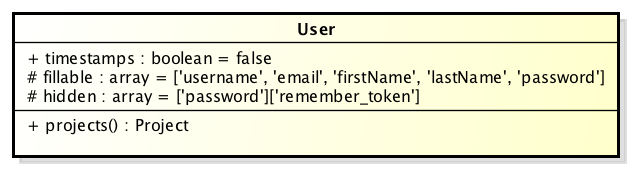
\includegraphics[width=0.8\linewidth]{img/back_end_user_model}
		\caption[Premi::Back-End::Model::User]{Premi::Back-End::Model::User}
		\label{fig:back_end_user_model}
	\end{figure}


	\paragraph{Descrizione:}
	Il modello User permette di gestire la collezione users del \gls{database}, relativa agli utenti registrati. Eloquent presume che il nome della classe sia il singolare del nome della collezione nel \gls{database}, quindi collega User alla collezione users.

	\paragraph{Utilizzo:}
	Il modello gestisce la collezione users del \gls{database}.
	
	\paragraph{Attributi:}
	\begin{itemize}
		\item \textbf{+ timestamps : boolean = false :}\\
		Di default Eloquent automatizza l'inserimento del timestamp relativo all'inserimento e aggiornamento di un campo. Se alla variabile viene assegnato il valore \textit{false} le informazioni dell'inserimento e del aggiornamento non verranno aggiunte alla collezione.
		\item \textbf{\# fillable : array = ['username', 'email', 'firstName', 'lastName', 'password']:}\\
		Quando si crea un modello, si deve passare una serie di attributi al costruttore del modello stesso. Questi attributi vengono assegnati al modello tramite \textbf{mass assignment}. La proprietà \textit{fillable} serve a specificare quali attributi devono essere assegnabili tramite il \textbf{mass assignment}.
		\begin{itemize}
			\item \textbf{username:} indica il nome utente scelto dall'utente;
			\item \textbf{email:} indica l'indirizzo email inserito dall'utente;
			\item \textbf{firstName:} indica il nome inserito dall'utente;
			\item \textbf{lastName:} indica il cognome inserito dall'utente;
			\item \textbf{password:} indica la password scelta dall'utente.
		\end{itemize}
	\end{itemize}
	
	\paragraph{Metodi:}
	\begin{itemize}
		\item \textbf{+ projects() : Project}\\
		Abbiamo utilizzato la relazione \textit{embedsMany} per riuscire ad incorporare il modello Project all'interno dell'oggetto principale User. Il metodo ritorna Project su cui verrà chiamato il metodo \textit{save()} nel caso in cui si voglia aggiornare il modello;
	\end{itemize}
\newpage

\subsubsection{Project}

	\begin{figure}[h]
		\centering
		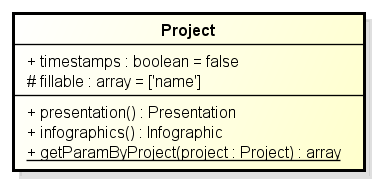
\includegraphics[width=0.5\linewidth]{img/back_end_premi_model_project}
		\caption[Premi::Back-End::Model::Project]{Premi::Back-End::Model::Project}
		\label{fig:back_end_premi_model_project}
	\end{figure}

	
	\paragraph{Descrizione:}
	Questa classe rappresenta un progetto di un utente.
	
	\paragraph{Utilizzo:}
	Viene utilizzata alla creazione di un progetto di un utente.
	
	\paragraph{Attributi:}
	\begin{itemize}
		\item \textbf{+ timestamps : boolean = false :}\\
		Di default Eloquent automatizza l'inserimento del timestamp relativo all'inserimento e aggiornamento di un campo. Se alla variabile viene assegnato il valore \textit{false} le informazioni dell'inserimento e del aggiornamento non verranno aggiunte alla collezione;
		\item \textbf{\# fillable : array = [’name’]:}\\
		Quando si crea un modello, si deve passare una serie di attributi al costruttore del modello stesso. Questi attributi vengono assegnati al modello tramite \textbf{mass assignment}. La proprietà \textit{fillable} serve a specificare quali attributi devono essere assegnabili tramite il \textbf{mass assignment}.
		\begin{itemize}
			\item \textbf{name:} indica il nome del progetto.
		\end{itemize}
	\end{itemize}
	
	\paragraph{Metodi:}
	\begin{itemize}
		\item \textbf{+ presentation() : Presentation}\\
		Abbiamo utilizzato la relazione \textit{embedsOne} per riuscire ad incorporare il modello Presentation all'interno dell'oggetto principale Project. Il metodo ritorna Presentation su cui verrà chiamato il metodo \textit{save()} nel caso in cui si voglia aggiornare il modello;
		\item \textbf{+ infographics() : Infographic}\\
		Abbiamo utilizzato la relazione \textit{embedsMany} per riuscire ad incorporare il modello Infographic all'interno dell'oggetto principale Project. Il metodo ritorna Infographic su cui verrà chiamato il metodo \textit{save()} nel caso in cui si voglia aggiornare il modello.
		\item \textbf{+ getParamByProject(project: Project) : array}\\
		La funzione riceve in ingresso una variabile di tipo Project e ne filtra i parametri che compongono tale oggetto restituendo un array contenente l'ID del progetto, il nome del progetto, l'ID della presentazione ad esso associato, il tema e la transizione della presentazione e la stringa SVG della prima slide della presentazione:\\
		\textbf{Argomenti:}
		\begin{itemize}
			\item project : Project;\\
			Progetto di cui si vogliono filtrare i parametri.
		\end{itemize}
	\end{itemize}

\newpage
\subsubsection{Infographic}

	\begin{figure}[h]
		\centering
		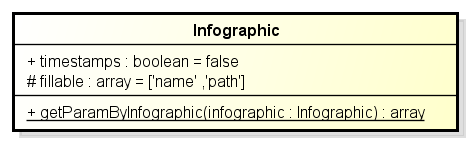
\includegraphics[width=0.5\linewidth]{img/back_end_premi_model_infographic}
		\caption[Premi::Back-End::Model::Infographic]{Premi::Back-End::Model::Infographic}
		\label{fig:back_end_premi_model_infographic}
	\end{figure}


	\paragraph{Descrizione:}
	Questa classe rappresenta un'\gls{infografica} di un progetto, ovvero una rappresentazione visuale della presentazione per mostrare in maniera semplice e veloce le informazioni.
	
	\paragraph{Utilizzo:}
	Viene utilizzata alla creazione di un'\gls{infografica} di una progetto.

	\paragraph{Attributi:}
		\begin{itemize}
			\item \textbf{+ timestamps : boolean = false :}\\
			Di default Eloquent automatizza l'inserimento del timestamp relativo all'inserimento e aggiornamento di un campo. Se alla variabile viene assegnato il valore \textit{false} le informazioni dell'inserimento e del aggiornamento non verranno aggiunte alla collezione;
			\item \textbf{\# fillable : array = [’name’, ’path’]:}\\
			Quando si crea un modello, si deve passare una serie di attributi al costruttore del modello stesso. Questi attributi vengono assegnati al modello tramite \textbf{mass assignment}. La proprietà \textit{fillable} serve a specificare quali attributi devono essere assegnabili tramite il \textbf{mass assignment}.
			\begin{itemize}
				\item \textbf{name:} indica il nome dell'\gls{infografica};
				\item \textbf{path:} indica il percorso dove recuperare il file dell'\gls{infografica}.
			\end{itemize}
		\end{itemize}
		
	\paragraph{Metodi:}
		\begin{itemize}
			\item \textbf{+ getParamByInfographic(infographic: Infographic) : array}\\
			La funzione riceve in ingresso una variabile di tipo Infographic e ne filtra i parametri che compongono tale oggetto restituendo un array contenente l'ID dell'infografica, il nome ed il path per recuperarla:\\
			\textbf{Argomenti:}
			\begin{itemize}
				\item infographic : Infographic;\\
				Infografica di cui si vogliono filtrare i parametri.
			\end{itemize}
		\end{itemize}
\newpage


\subsubsection{Presentation}

	\begin{figure}[h]
		\centering
		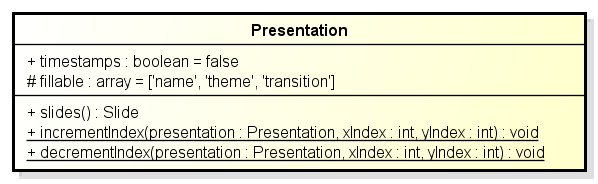
\includegraphics[width=0.8\linewidth]{img/back_end_premi_model_presentation}
		\caption[Premi::Back-End::Model::Presentation]{Premi::Back-End::Model::Presentation}
		\label{fig:back_end_premi_model_presentation}
	\end{figure}


	\paragraph{Descrizione:}
	Questa classe descrive la presentazione di un progetto. Contiene tutte le \textit{\gls{slide}} che servono a comporre la presentazione.

	\paragraph{Utilizzo}
	Viene utilizzato alla creazione o caricamento di una presentazione.
	
	\paragraph{Attributi:}
	\begin{itemize}
		\item \textbf{+ timestamps : boolean = false :}\\
		Di default Eloquent automatizza l'inserimento del timestamp relativo all'inserimento e aggiornamento di un campo. Se alla variabile viene assegnato il valore \textit{false} le informazioni dell'inserimento e del aggiornamento non verranno aggiunte alla collezione;
		\item \textbf{\# fillable : array = ['title', 'theme', 'transition']:}\\
		Quando si crea un modello, si deve passare una serie di attributi al costruttore del modello stesso. Questi attributi vengono assegnati al modello tramite \textbf{mass assignment}. La propietà \textit{fillable} serve a specificare quali attributi devono essere assegnabili tramite il \textbf{mass assignment}.
		\begin{itemize}
			\item \textbf{title:} indica il titolo della presentazione;
			\item \textbf{theme:} indica il tema, inteso come \textit{\gls{font}} e colore di sfondo, utilizzato per la presentazione;
			\item \textbf{transition:} indica il tipo di transizione da una \textit{\gls{slide}} all'altra durante la visualizzazione della presentazione.
		\end{itemize}
	\end{itemize}

	\paragraph{Metodi:}
	\begin{itemize}
		\item \textbf{+ slides() : Slide}\\
		Abbiamo utilizzato la relazione \textit{embedsMany} per riuscire ad incorporare il modello \gls{Slide} all’interno dell’oggetto principale Presentation. Il metodo ritorna \gls{Slide} su cui verrà chiamato il metodo \textit{save()} nel caso in cui si voglia aggiornare il modello.
		\item \textbf{+ incrementIndex(presentation: Presentation, xIndex: int, yIndex: int) : void}\\
		Tale metodo statico riceve in input un oggetto di tipo Presentation ed i valori degli assi X e Y dove verrà inserita la nuova \gls{slide}. Il metodo utilizza una query per ritornare l'insieme delle \gls{slide} che devono essere traslate a causa dell'inserimento della nuova \gls{slide}, e, per ognuna, effettua un incremento dei valori degli assi X e Y in base alla nuova posizione che dovrà occupare la \gls{slide}:\\
		\textbf{Argomenti:}
		\begin{itemize}
			\item presentation : Presentation;\\
			Presentazione di cui si vogliono incrementare gli indici delle \gls{slide}.
			\item xIndex : int;\\
			Indice dell'asse X della \gls{slide} appena inserita, da cui, se necessario, bisogna partire a fare l'incremento.
			\item yIndex : int;\\
			Indice dell'asse Y della \gls{slide} appena inserita, da cui, se necessario, bisogna partire a fare l'incremento.
		\end{itemize}
		\item \textbf{+ decrementIndex(presentation: Presentation, xIndex: int, yIndex: int) : void}\\
		Tale metodo statico riceve in input un oggetto di tipo Presentation ed i valori degli assi X e Y della \gls{slide} appena cancellata. Il metodo utilizza una query per ritornare l'insieme delle \gls{slide} che devono essere traslate a causa della cancellazione della nuova \gls{slide}, e, per ognuna, effettua un decremento dei valori degli assi X e Y in base alla nuova posizione che dovrà occupare la \gls{slide}:\\
		\textbf{Argomenti:}
		\begin{itemize}
			\item presentation : Presentation;\\
			Presentazione di cui si vogliono decrementare gli indici delle \gls{slide}.
			\item xIndex : int;\\
			Indice dell'asse X della \gls{slide} appena inserita, da cui, se necessario, bisogna partire a fare il decremento.
			\item yIndex : int;\\
			Indice dell'asse Y della \gls{slide} appena inserita, da cui, se necessario, bisogna partire a fare decremento.
		\end{itemize}
	\end{itemize}
\newpage


\subsubsection{Slide}

	\begin{figure}[h]
		\centering
		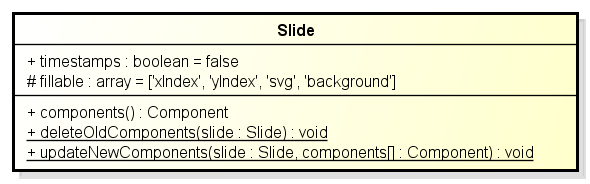
\includegraphics[width=0.7\linewidth]{img/back_end_premi_model_slide}
		\caption[Premi::Back-End::Model::Slide]{Premi::Back-End::Model::Slide}
		\label{fig:back_end_premi_model_slide}
	\end{figure}


	\paragraph{Descrizione:}
	Questa classe descrive una singola \gls{slide}. Contiene tutti i gli oggetti appartenenti alla \gls{slide}.
	
	\paragraph{Utilizzo:}
	Viene utilizzato alla creazione o caricamento di una \gls{slide}.

	\paragraph{Attributi:}
	\begin{itemize}
		\item \textbf{+ timestamps : boolean = false :}\\
		Di default Eloquent automatizza l'inserimento del timestamp relativo all'inserimento e aggiornamento di un campo. Se alla variabile viene assegnato il valore \textit{false} le informazioni dell'inserimento e del aggiornamento non verranno aggiunte alla collezione;
		\item \textbf{\# fillable : array = [’xIndex’, ’yIndex', 'svg', 'background']:}\\
		Quando si crea un modello, si deve passare una serie di attributi al costruttore del modello stesso. Questi attributi vengono assegnati al modello tramite \textbf{mass assignment}. La proprietà \textit{fillable} serve a specificare quali attributi devono essere assegnabili tramite il \textbf{mass assignment}.
		\begin{itemize}
			\item \textbf{xIndex:} indica la posizione relativa all'asse X delle \gls{slide} nella matrice di \gls{slide} della presentazione;
			\item \textbf{yIndex:} indica la posizione relativa all'asse Y delle \gls{slide} nella matrice di \gls{slide} della presentazione;
			\item \textbf{svg:} specifica l'attributo che identifica la stringa SVG relativa alla \gls{slide};
			\item \textbf{background:} indica il colore di sfondo di una \gls{slide}.
		\end{itemize}
	\end{itemize}
	
	\paragraph{Metodi:}
	\begin{itemize}
		\item \textbf{+ components() : Component}\\
		Abbiamo utilizzato la relazione \textit{embedsMany} per riuscire ad incorporare il modello Component all'interno dell'oggetto principale \gls{Slide}. Il metodo ritorna Component su cui verrà chiamato il metodo \textit{save()} nel caso in cui si voglia aggiornare il modello.
		\item \textbf{+ deleteOldComponents(slide: Slide) : void}\\
		Questo metodo statico riceve in ingresso un oggetto di tipo \gls{Slide}, ed elimina tutti i vecchi componenti di tale \gls{slide} prima di effettuare l'aggiornamento con i nuovi componenti:\\
		\textbf{Argomenti:}
		\begin{itemize}
			\item \gls{slide} : \gls{Slide};\\
			\gls{Slide} di cui eliminare i componenti.
		\end{itemize}
		\newpage
		\item \textbf{+ updateNewComponents(slide: Slide, components[]: Component) : void}\\
		Questo metodo statico riceve in ingresso un oggetto di tipo \gls{Slide} ed un array di Component ed inserisce nella \gls{slide} tutti i nuovi componenti presenti nell'array:\\
		\textbf{Argomenti:}
		\begin{itemize}
			\item slide : Slide;\\
			\gls{Slide} di cui si vogliono aggiornare i componenti.
			\item components[] : Component;\\
			Array di componenti da inserire nella \gls{slide}.
		\end{itemize}
		\item \textbf{+ getComponentsBySlide(slide: Slide) : array}\\
		La funzione riceve in ingresso una variabile di tipo Slide e ne filtra i parametri che compongono tale oggetto restituendo un array contenente l'ID della \gls{slide}, la sua posizione rispetto agli assi X e Y della matrice della presentazione e la sua collezione di componenti:\\
		\textbf{Argomenti:}
		\begin{itemize}
			\item slide : Slide;\\
			\gls{Slide} di cui si vogliono filtrare i parametri.
		\end{itemize}
		\item \textbf{+ getSVGBySlides(slide: Slide) : array}\\
		La funzione riceve in ingresso una variabile di tipo Slide e ne filtra i parametri che compongono tale oggetto restituendo un array contenente l'ID della \gls{slide}, la sua posizione rispetto agli assi X e Y della matrice della presentazione e la sua stringa SVG:\\
		\textbf{Argomenti:}
		\begin{itemize}
			\item slide : Slide;\\
			\gls{Slide} di cui si vogliono filtrare i parametri.
		\end{itemize}
	\end{itemize}
	\newpage
	

\subsubsection{Component}

	\begin{figure}[h]
		\centering
		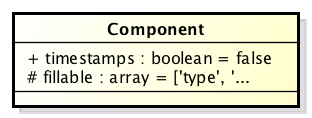
\includegraphics[width=0.5\linewidth]{img/back_end_premi_model_component}
		\caption[Premi::Back-End::Model::Component]{Premi::Back-End::Model::Component}
		\label{fig:back_end_premi_model_component}
	\end{figure}


	\paragraph{Descrizione:}
	Questa classe descrive la struttura generica di un componente.
	
	\paragraph{Utilizzo:}
	Viene utilizzato alla creazione o caricamento di una componente.
	
	\paragraph{Attributi:}
	\begin{itemize}
		\item \textbf{+ timestamps : boolean = false :}\\
		Di default Eloquent automatizza l'inserimento del timestamp relativo all'inserimento e aggiornamento di un campo. Se alla variabile viene assegnato il valore \textit{false} le informazioni dell'inserimento e del aggiornamento non verranno aggiunte alla collezione;
		\item \textbf{\# fillable : array = [’type’, ’originX’, ’OriginY’, ’left’, ’top’, ’width’, ’height’, ’fill’, ’stroke’, ’strokeWidth’, ’strokeDashArray’, ’strokeLineCap’, ’strokeLine-Join’, ’strokeMiterLimit’, ’scaleX’, ’scaleY’, ’angle’, ’flipX’, ’flipY’, ’opacity’, ’shadow’, ’visible’, ’clipTo’, ’backgroundColor’, ’fillRule’, ’globalCompositeOperation']:}\\
		Quando si crea un modello, si deve passare una serie di attributi al costruttore del modello stesso. Questi attributi vengono assegnati al modello tramite \textbf{mass assignment}. La proprietà \textit{fillable} serve a specificare quali attributi devono essere assegnabili tramite il \textbf{mass assignment}.
		\begin{itemize}
			\item \textbf{type:} indica il tipo di componente;
			\item \textbf{originX:} indica la posizione relativa all'asse X del vertice d'origine del componente;
			\item \textbf{originY:} indica la posizione relativa all'asse Y del vertice d'origine del componente;
			\item \textbf{left:} indica la posizione relativa all'asse delle X dell'area di disegno in cui verrà disegnato il componente;
			\item \textbf{top:} indica la posizione relativa all'asse delle Y dell'area di disegno in cui verrà disegna il componente;
			\item \textbf{width:} larghezza del riquadro che racchiude il componente;
			\item \textbf{height:} altezza del riquadro che racchiude il componente;
			\item \textbf{fill:} indica il colore di riempimento del riquadro che racchiude il componente;
			\item \textbf{stroke:} indica il colore del tratto utilizzato per disegnare il componente;
			\item \textbf{strokeWidth:} indica la larghezza del tratto utilizzato per disegnare il componente;
			\item \textbf{strokeDashArray:} indica il tipo di tratto utilizzato per disegnare il componente;
			\item \textbf{strokeLineCap:} indica lo stile di fine del tratto utilizzato per disegnare il componente;
			\item \textbf{strokeLine-Join:} indica lo stile degli angoli del tratto utilizzato per disegnare il componente;
			\item \textbf{strokeMiterLimit:} indica il limite della distanza di unione tra due linee;
			\item \textbf{scaleX:} indica il valore con cui viene scalato in larghezza il componente;
			\item \textbf{scaleY:} indica il valore con cui viene scalato in altezza il componente;
			\item \textbf{angle:} indica l'angolo di rotazione del componente;
			\item \textbf{flipX:} indica se il componente è capovolto rispetto all'asse X;
			\item \textbf{flipY:} indica se il componente è capovolto rispetto all'asse Y;
			\item \textbf{opacity:} indica il livello di opacità del componente;
			\item \textbf{shadow:} indica il livello dell'ombra del componente;
			\item \textbf{visible:} indica  se il componente è visibile o no;
			\item \textbf{clipTo:} indica se il componente ha l'effetto clip attivo;
			\item \textbf{backgroundColor:} indica il colore di sfondo del componente;
			\item \textbf{fillRule:} indica lo stile di riempimento;
			\item \textbf{globalCompositeOperation:} indica l'ordine in cui vengono disegnati i componenti all'interno di un gruppo.
		\end{itemize}
	\end{itemize}
\newpage

\subsubsection{Chart}

	\begin{figure}[h]
		\centering
		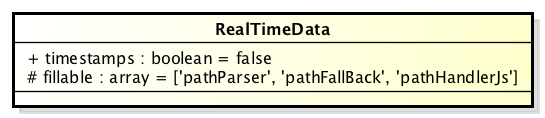
\includegraphics[width=0.5\linewidth]{img/back_end_premi_model_realTimeData}
		\caption[Premi::Back-End::Model::Chart]{Premi::Back-End::Model::Chart}
		\label{fig:back_end_premi_model_chart}
	\end{figure}

	\paragraph{Descrizione}
	Questa classe rappresenta la struttura di dati necessari per descrivere un grafico all'interno di una \gls{slide}. Tale classe estende la classe Component.
	
	\paragraph{Utilizzo}
	Viene utilizzato alla creazione o caricamento di un grafico.

	\paragraph{Attributi}
	\begin{itemize}
		\item \textbf{+ timestamps : boolean = false :}\\
		Di default Eloquent automatizza l'inserimento del timestamp relativo all'inserimento e aggiornamento di un campo. Se alla variabile viene assegnato il valore \textit{false} le informazioni dell'inserimento e del aggiornamento non verranno aggiunte alla collezione.
		\item \textbf{\# fillable : array = [’typeChart’ , ’data’]:}\\
		Quando si crea un modello, si deve passare una serie di attributi al costruttore del modello stesso. Questi attributi vengono assegnati al model tramite \textbf{mass assignment}. La proprietà \textit{fillable} serve a specificare quali attributi devono essere assegnabili tramite il \textbf{mass assignment}.
		\begin{itemize}
			\item \textbf{typeChart:} indica il tipo di grafico;
			\item \textbf{data:} indica l'array di dati che servono a comporre il grafico.
		\end{itemize}
		
	\end{itemize}
\newpage


\subsubsection{RealTimeData}

	\begin{figure}[h]
		\centering
		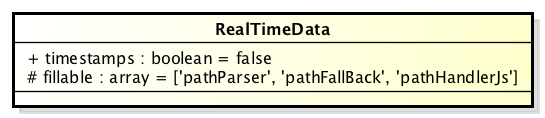
\includegraphics[width=0.5\linewidth]{img/back_end_premi_model_realTimeData}
		\caption[Premi::Back-End::Model::RealTimeData]{Premi::Back-End::Model::RealTimeData}
		\label{fig:back_end_premi_model_realTimeData}
	\end{figure}


	\paragraph{Descrizione}
	Questa classe rappresenta la struttura di dati necessari per descrivere RealTimeData (dato in tempo reale) all'interno di una \gls{slide}. Tale classe estende la classe Component.
	
	\paragraph{Utilizzo}
	Viene utilizzato alla creazione o caricamento di un RealTimeData.
	
	\paragraph{Attributi}
	\begin{itemize}
		\item \textbf{+ timestamps : boolean = false :}\\
		Di default Eloquent automatizza l'inserimento del timestamp relativo all'inserimento e aggiornamento di un campo. Se alla variabile viene assegnato il valore \textit{false} le informazioni dell'inserimento e del aggiornamento non verranno aggiunte alla collection.
		\item \textbf{\# fillable : array = ['pathParser’, ’pathFallback’, ’pathHandlerJs']:}\\
		Quando si crea un modello, si deve passare una serie di attributi al costruttore del model stesso. Questi attributi vengono assegnati al modello tramite \textbf{mass assignment}. La proprietà \textit{fillable} serve a specificare quali attributi devono essere assegnabili tramite il \textbf{mass assignment}.
		\begin{itemize}
			\item \textbf{pathParser:} Indirizzo del \gls{parser} \gls{php} \footnote{file \gls{php} con il compito di recuperare i dati da un indirizzo remoto (evitando cosi il problema della same-origin-policy) fornendo come risultato un oggetto \gls{JSON} che sarà poi processato dall'Handler \gls{javascript}};
			\item \textbf{pathFallback:} Indirizzo del file contenente l'oggetto più recente salvato in caso di consultazione offline;
			\item \textbf{pathHandlerJs:} Indirizzo del handler \gls{javascript} con il compito di impaginare i risultati provenienti dal \gls{parser} e riaggiornare la vista dopo n secondi.
		\end{itemize}
	\end{itemize}
\newpage


\subsubsection{Text}

	\begin{figure}[h]
		\centering
		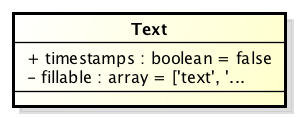
\includegraphics[width=0.5\linewidth]{img/back_end_premi_model_text}
		\caption[Premi::Back-End::Model::Text]{Premi::Back-End::Model::Text}
		\label{fig:back_end_premi_model_text}
	\end{figure}


	\paragraph{Descrizione}
	Questa classe rappresenta la struttura di dati di un campo di testo di una \gls{slide}. Tale classe estende la classe Component.
	
	\paragraph{Utilizzo}
	Viene utilizzato alla creazione o caricamento di un campo di testo.
	
	\paragraph{Attributi}
	\begin{itemize}
		\item \textbf{+ timestamps : boolean = false :}\\
		Di default Eloquent automatizza l'inserimento del timestamp relativo all'inserimento e aggiornamento di un campo. Se alla variabile viene assegnato il valore \textit{false} le informazioni dell'inserimento e del aggiornamento non verranno aggiunte alla collezione.
		\item \textbf{\# fillable : array = [’text’, ’fontSize’, ’fontWeight’, ’fontFamily’, ’fontStyle’, ’lineHeight’, ’textDecoration’, ’textAlign’, ’textBackgroundColor']:}\\
		Quando si crea un modello, si deve passare una serie di attributi al costruttore del modello stesso. Questi attributi vengono assegnati al modello tramite \textbf{mass assignment}. La proprietà \textit{fillable} serve a specificare quali attributi devono essere assegnabili tramite il \textbf{mass assignment}.
		\begin{itemize}
			\item \textbf{text:} indica il contenuto del campo di testo;
			\item \textbf{fontSize:} indica le dimensioni del \gls{font} del campo di testo;
			\item \textbf{fontWeight:} indica lo spessore del testo;
			\item \textbf{fontFamily:} indica la famiglia di \gls{font} del campo di testo;
			\item \textbf{fontStyle:} indica lo stile del \gls{font} del campo di testo (corsivo, grassetto, sottolineato);
			\item \textbf{lineHeight:} indica l'altezza della linea del campo di testo;
			\item \textbf{textDecoration:} indica il tipo di decorazione;
			\item \textbf{textAlign:} indica l'allineamento del testo all'interno del campo di testo;
			\item \textbf{textBackgroundColor:} indica il colore di sfondo del campo di testo.
		\end{itemize}
	\end{itemize}
\newpage


\subsubsection{Image}

	\begin{figure}[h]
		\centering
		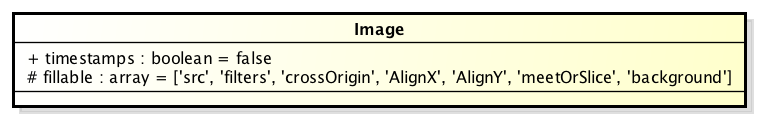
\includegraphics[width=0.8\linewidth]{img/back_end_premi_model_image}
		\caption[Premi::Back-End::Model::Image]{Premi::Back-End::Model::Image}
		\label{fig:back_end_premi_model_image}
	\end{figure}


	\paragraph{Descrizione}
	La classe Image rappresenta la struttura dei dati necessari per rappresentare un'immagine all'interno di una \gls{slide}. Tale classe estende la classe Component.
	
	\paragraph{Utilizzo}
	Utilizzata quando viene inserita un'immagine per tenerne traccia.
	
	\paragraph{Attributi}
	\begin{itemize}
		\item \textbf{+ timestamps : boolean = false :}\\
		Di default Eloquent automatizza l'inserimento del timestamp relativo all'inserimento e aggiornamento di un campo. Se alla variabile viene assegnato il valore \textit{false} le informazioni dell'inserimento e del aggiornamento non verranno aggiunto alla collezione.
		\item \textbf{\# fillable : array = [’src’, ’filters’, ’crossOrigin’, ’alignX’, ’alignY’,’meetOrSlice’, ’background’]:}\\
		Quando si crea un modello, si deve passare una serie di attributi al costruttore del modello stesso. Questi attributi vengono assegnati al modello tramite \textbf{mass assignment}. La proprietà \textit{fillable} serve a specificare quali attributi devono essere assegnabili tramite il \textbf{mass assignment}.
		\begin{itemize}
			\item \textbf{src:} indica il percorso dove recuperare il file dell'immagine;
			\item \textbf{filters:} indica quali filtri verranno applicati all'immagine;
			\item \textbf{crossOrigin:} utilizzato per passare informazioni assieme all'immagine;
			\item \textbf{alignX:} indica l'allineamento relativo all'asse X dell'immagine;
			\item \textbf{alignY:} indica l'allineamento relativo all'asse Y dell'immagine;
			\item \textbf{meetOrSlice:} indica se l'immagine dev'essere tagliata quando la sua finestra si restringe o essere sempre completamente visibile;
			\item \textbf{background:} indica lo sfondo dell'immagine.
		\end{itemize}
	\end{itemize}
\newpage


\subsubsection{Table}

	\begin{figure}[h]
		\centering
		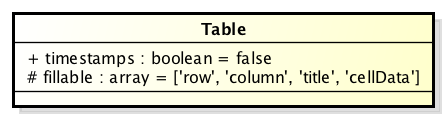
\includegraphics[width=0.5\linewidth]{img/back_end_premi_model_table}
		\caption[Premi::Back-End::Model::Table]{Premi::Back-End::Model::Table}
		\label{fig:back_end_premi_model_table}
	\end{figure}


	\paragraph{Descrizione}
	Questa classe rappresenta la struttura di dati di una tabella di una \gls{slide}. Tale classe estende la classe Component.
	
	\paragraph{Utilizzo}
	Viene utilizzato alla creazione o caricamento di una tabella.
	
	\paragraph{Attributi}
	\begin{itemize}
		\item \textbf{+ timestamps : boolean = false :}\\
		Di default Eloquent automatizza l'inserimento del timestamp relativo all'inserimento e aggiornamento di un campo. Se alla variabile viene assegnato il valore le informazioni dell'inserimento e del aggiornamento non verranno aggiunto alla collezione.
		\item \textbf{\# fillable : array = [’row’, ’column’, ’title’, ’cellData’]:}\\
		Quando si crea un modello, si deve passare una serie di attributi al costruttore del modello stesso. Questi attributi vengono assegnati al modello tramite \textbf{mass assignment}. La proprietà \textit{fillable} serve a specificare quali attributi devono essere assegnabili tramite il \textbf{mass assignment}.
		\begin{itemize}
			\item \textbf{row:} indica il numero di righe della tabella;
			\item \textbf{column:} indica il numero di colonne della tabella;
			\item \textbf{title:} indica il titolo della tabella;
			\item \textbf{cellData:} indica l'array di dati necessario a comporre la tabella.
		\end{itemize}
	\end{itemize}
